\documentclass[11pt,a4paper,fleqn]{scrartcl}

\usepackage[utf8]{inputenc}
\usepackage[T1]{fontenc}
\usepackage[colorlinks=true, citecolor=blue, linkcolor=blue, filecolor=blue,urlcolor=blue]{hyperref}
\hypersetup{
	colorlinks   = true,
	citecolor    = gray
}
\usepackage{wrapfig}

\usepackage{caption}
\captionsetup{format=plain, indent=5pt, font=footnotesize, labelfont=bf}

\setkomafont{disposition}{\scshape\bfseries}

\usepackage{amsmath}
\usepackage{amssymb}
\usepackage{amsfonts}
\usepackage{bbm}
\usepackage{mathtools}
% \usepackage{epsfig}
% \usepackage{grffile}
%\usepackage{times}
%\usepackage{babel}
\usepackage{tikz}
\usepackage{paralist}
\usepackage{color}
\usepackage[top=3cm, bottom=2.5cm, left=2.5cm, right=3cm]{geometry}
%\setlength{\mathindent}{1ex}
\usepackage{fontawesome}
% PGF
\usepackage{pgfplots}
\usepackage{pgf}
\usepackage{siunitx}
\usepackage{xfrac}
\usepackage{calculator}
\usepackage{calculus}
\usepackage{eurosym}
\usepackage{booktabs}
%\sisetup{per-mode=fraction,%
%	fraction-function=\sfrac}

%\newcommand{\eur}[1]{\EUR{#1}\si{\per\kilo\meter}}
\pgfplotsset{
	compat=newest,
	every axis/.append style={small, minor tick num=3}
}

%\usepackage[backend=biber,style=alphabetic,url=false,doi=false]{biblatex}
%\addbibresource{sheet01_biber.bib}
% \addbibresource{/home/coroa/papers/refs.bib}

\newcommand{\id}{\mathbbm{1}}
\newcommand{\NN}{{\mathbbm{N}}}
\newcommand{\ZZ}{{\mathbbm{Z}}}
\newcommand{\RR}{{\mathbbm{R}}}
\newcommand{\CC}{{\mathbbm{C}}}
\renewcommand{\vec}[1]{{\boldsymbol{#1}}}

\renewcommand{\i}{\mathrm{i}}

\newcommand{\expect}[1]{\langle\,#1\,\rangle}
\newcommand{\e}[1]{\ensuremath{\,\mathrm{#1}}}

\renewcommand{\O}{\mc{O}}
\newcommand{\veps}{\varepsilon}
\newcommand{\ud}[1]{\textup{d}#1\,}

\newcommand{\unclear}[1]{\color{green}#1}
\newcommand{\problem}[1]{\color{red}#1}
\newcommand{\rd}[1]{\num[round-mode=places,round-precision=1]{#1}}

%\DeclareSIUnit{\euro}{\EUR}
\DeclareSIUnit{\dollar}{\$}
\newcommand{\eur}{\text{\EUR{}}}

\usepackage{palatino}
\usepackage{mathpazo}
\setlength\parindent{0pt}
\usepackage{xcolor}
\usepackage{framed}
\definecolor{shadecolor}{rgb}{.9,.9,.9}

\def\cap{\text{Cap}}
\def\floor{\text{Floor}}
\def\l{\lambda}
\def\m{\mu}
\def\d{\partial}
\def\cL{\mathcal{L}}
\def\co2{CO${}_2$}

\def\mw{\text{ MW}}
\def\mwh{\text{ MWh}}
\def\gw{\text{ GW}}
\def\gwh{\text{ GWh}}
\def\emwh{\text{ \euro/MWh}}
\def\bemwh{\text{ [\euro/MWh]}}

%=====================================================================
%=====================================================================
\begin{document}

\begin{flushright}
 \textbf{Energy System Modelling }\\
 {\small Karlsruhe Institute of Technology}\\
 {\small Institute for Automation and Applied Informatics}\\
 {\small Summer Term 2020}\\
\end{flushright}

 
 \vspace{-0.5em}
 \hrulefill
 \vspace{0.3em}

\begin{center}
 \textbf{\textsc{\Large Tutorial IV: Electricity Markets}}\\
 \small Will be worked on in the exercise session on Thursday, 25 June 2020.\\[1.5em]
\end{center}

\vspace{-0.5em}
\hrulefill
\vspace{0.8em}

%=============== ======================================================
\paragraph{Problem IV.1 (analytical) -- shadow prices \faGroup}~\\
%=====================================================================

Suppose that the utility for the electricity consumption of an industrial company is given by
\[
 U(d) = 70d - 3d^2 ~[\textrm{\euro}/\si{\mega\watt\hour}] \quad , \quad d\in [d_{min},d_{max}]=[2,10],
\]
where $d$ is the demand in MW and $d_{min}, d_{max}$ are the minimum and maximum demand. \\
[1em]
Assume that the company is maximising its net surplus for a given electricity price $\pi$, i.e. it maximises $\max_{d} \left[U(d) -
  \pi d\right]$.
\begin{enumerate}[(a)]
 \item  If the price is $\pi = 5$~\euro/MWh, what is the optimal
       demand $d^*$?  What is the value of the KKT multiplier $\mu_{max}$
       for the constraint $d \leq d_{max}=10$ at this optimal solution?
       What is the value of $\mu_{min}$ for $d \geq d_{min} = 2$?
 \item Suppose now the electricity price is $\pi = 60$~\euro/MWh. What are
       the optimal demand $d^*$, $\mu_{max}$ and $\mu_{min}$ now?
\end{enumerate}

%=============== ======================================================
\paragraph{Problem IV.2 (analytical) -- Economic dispatch in a single bidding zone \faGroup}~\\
%=====================================================================

Consider an electricity market with two generator types, one with the cost function $C_1(g_1)=c_1g_1$ with variable cost $c_1 = 20\emwh$, capacity $G_1 = 300\mw$ and a dispatch rate of $g_1$~[MW], and another with the cost function $C_2(g_2)=c_2g_2$ with variable cost $c_2=50\emwh$, capacity $G_2=400\mw$ and a dispatch rate of $g_2$~[MW]. The demand-side has utility function $U(d) = 8000d - 5d^2$~[\euro/h] for a consumption rate of $d$~[MW].
\begin{enumerate}[(a)]
 \item What are the objective function and constraints required for an optimisation problem to maximise short-run social welfare in this market?
 \item Write down the Karush-Kuhn-Tucker (KKT) conditions for this problem.
 \item Determine the optimal rate of production of the generators and the value of all KKT multipliers. What is the interpretation of the respective KKT multipliers?
\end{enumerate}

\newpage
%=============== ======================================================
\paragraph{Problem IV.3 (analytical) -- efficient dispatch in a two-bus power system \faHome}~\\
%=====================================================================

\begin{figure}[h]
 \centering
 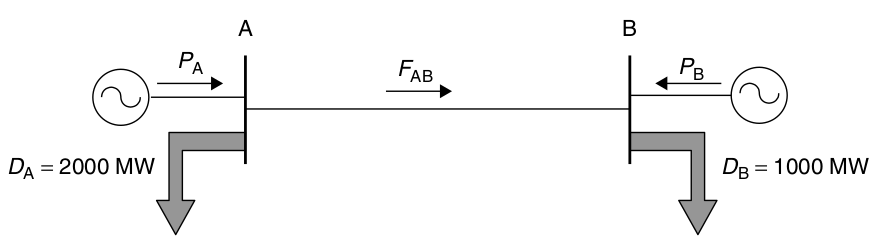
\includegraphics[width=14cm]{two-bus}

 \caption{A simple two-bus power system.}
 \label{twobus}
\end{figure}

Consider the two-bus power system shown in Figure \ref{twobus}, where the two nodes represent two markets, each with different total demand $D_i$, and one generator at each node producing $P_i$. At node A the demand is $D_A = 2000 \si{\mega\watt}$, whereas at node B the demand is $D_B = 1000 \si{\mega\watt}$. Furthermore, there is a transmission line with a capacity denoted by $F_{AB}$. The marginal cost of production of the generators connected to buses A and B are given respectively by the following expressions:

\begin{align*}
 MC_A & = 20 + 0.03 P_A \hspace{1cm}\eur/\si{\mega\watt\hour}  \\
 MC_B & = 15 + 0.02 P_B \hspace{1cm} \eur/\si{\mega\watt\hour}
\end{align*}

Assume that the demands $D_A$ and $D_B$ are constant and insensitive to price, that energy is sold at its marginal cost of production and that there are no limits on the output of the generators.

\begin{enumerate}[(a)]
 \item Calculate the price of electricity at each bus, the production
       of each generator, and the flow on the line for the following cases. You may also calculate the values of any KKT multiplier as a bonus.
       \begin{enumerate}[(i)]
        \item The line between buses A and B is disconnected.
        \item The line between buses A and B is in service and has an unlimited capacity.
        \item The line between buses A and B is in service and has an unlimited capacity, but the maximum output of Generator B is 1500~MW.
        \item The   line between buses A and B is in service and has an unlimited capacity, but the maximum output of Generator A is 900~MW. The output of Generator B is unlimited.
        \item The line between buses A and B is in service but its capacity is limited to 600~MW. The output of the generators is unlimited.
       \end{enumerate}
 \item Calculate the generator revenues, generator profits, consumer payments and consumer net surplus for all the cases considered in the above problem. Who benefits from the line connecting these two buses?
 \item Calculate the congestion surplus for case (v). For what values of the flow on the line between buses A and B is the congestion surplus equal to zero?
\end{enumerate}

\end{document}
